\PassOptionsToPackage{hyphens}{url}
\documentclass[11pt,a4paper]{article}
\usepackage[T1]{fontenc}
\usepackage[utf8]{inputenc}
\usepackage[spanish,es-noquoting,es-tabla]{babel}
\usepackage{amsmath,amssymb}
\usepackage{booktabs}
\usepackage{graphicx}
\usepackage[margin=2.4cm]{geometry}
\usepackage{microtype}
\usepackage[colorlinks=true,linkcolor=black,urlcolor=blue,citecolor=black]{hyperref}
\usepackage{xcolor}
\urlstyle{tt}
\usepackage{enumitem}
\usepackage{tocloft}
\setlength{\cftsecnumwidth}{2.4em}
\setlength{\cftsubsecnumwidth}{3.2em}
\setlist{nosep}

\newcommand{\avg}[1]{\langle #1\rangle}
\newcommand{\dd}{\mathrm{d}}
\newcommand{\etq}[1]{\textcolor{gray}{\texttt{[#1]}}}
\newcommand{\repo}{\href{https://github.com/Lucia-Maz/free-slip-boundary-conditions-fourier-continuation}{\texttt{Lucia-Maz/free-slip-boundary-conditions-fourier-continuation}}}
\graphicspath{{../salidas/figuras/}}

\title{Fricción de fondo de una capa delgada con superficie libre:\\
la condición \emph{free-slip} en SPECTER}
\author{Lucía Mazaira\\ \small INFINA, CONICET--UBA}
\date{\small Ondas Gravitacionales e Investigación Asistida por IA --- entrega, 17 de septiembre de 2026}

\begin{document}
\maketitle

\begin{abstract}
\noindent
La fricción con el fondo domina el decaimiento de una capa delgada de fluido, y en las
simulaciones cuasi-2D entra como un coeficiente $\alpha$ ajustado, porque los códigos o no
tienen bordes o los tienen no-deslizantes de los dos lados. Este trabajo implementa en
SPECTER ---pseudoespectral con continuación de Fourier, no periódico en $z$--- la condición
de superficie libre no deformable (\emph{free-slip}: cara plana sin tensión tangencial) y la
verifica contra una referencia independiente; con ella $\alpha$ se \emph{calcula}:
$\alpha=\nu\pi^2/4h^2$, exactamente cuatro veces menor que con tapa rígida, reproducido por
el código con error $6{,}8\cdot10^{-10}$. Con el mismo código se mide qué hace la no
linealidad: sube la fricción de fondo hasta $26\%$ en $\delta=10$, pero la velocidad de
superficie ---lo que un PIV ajusta--- decae más lento que el promedio vertical, y en el
régimen de la ventana experimental las dos correcciones casi se cancelan. El decaimiento
medido por PIV en la celda de forzado electromagnético da $\alpha=0{,}0669\pm0{,}0049\,
\mathrm{s^{-1}}$ contra $0{,}0685$ calculado y $0{,}274$ de tapa rígida, con una salvedad
cuantitativa abierta que se declara. Todo número de este documento apunta a un chequeo
ejecutable, un script con su JSON o una entrada del log de decisiones del repositorio
\repo.
\end{abstract}

\tableofcontents

\section{La pregunta}

En las simulaciones de turbulencia cuasi-2D que usa el grupo, el decaimiento de una capa
delgada de fluido está dominado por la fricción con el fondo. Esa fricción nace de una
asimetría: el fondo es no-deslizante y la superficie de arriba es libre (el electrolito
está en contacto con aire). Los códigos existentes o no tienen bordes verticales
(periódicos en $z$), o los tienen no-deslizantes de los dos lados; en cualquiera de los dos
casos la fricción entra como un término $-\alpha\boldsymbol U$ con un $\alpha$ ajustado, no
calculado.

La pregunta del proyecto es si $\alpha$ se puede \emph{calcular} a partir de la condición
de contorno real, y qué le hace la no linealidad. Para eso se implementó en SPECTER
\cite{fontana2020} la condición de superficie libre en la cara superior, se verificó, se
usó para medir $\alpha$ en régimen no lineal, y se contrastó con un decaimiento medido.

Las etiquetas \etq{D-nn} (decisión), \etq{H-nn} (hallazgo), \etq{V-nn} (verificación) y
\etq{P-nn} (pregunta abierta) resuelven en \texttt{DECISIONES.md} del repositorio, que es
el log completo: qué se decidió, por qué, qué alternativa se descartó y qué salió mal.
Este documento es la lectura explicada; la página HTML es el resumen.

\section{La superficie libre: qué se implementa y por qué vale}
\label{sec:superficie}

\subsection{Las condiciones físicas y su orden cero}

Una superficie libre real, en $z=h+\eta(x,y,t)$, impone tres cosas sobre el fluido:
\begin{enumerate}
  \item \textbf{tensión tangencial nula}: el aire no arrastra;
  \item \textbf{condición cinemática}: la superficie se mueve con el fluido,
        $w(h)=\partial_t\eta+\boldsymbol u_h\cdot\nabla_h\eta$;
  \item \textbf{balance de tensión normal}: la presión en la superficie está fijada por lo
        que la restituye, $p(h)=\rho g\eta-\sigma\nabla_h^2\eta+2\mu\,\partial_z w|_h$.
\end{enumerate}
Si la deformación es chica frente al espesor, $\eta\ll h$, las dos últimas colapsan a
$w=0$ sobre el plano fijo $z=h$, y lo que queda es una \emph{cara plana sin tensión
tangencial}:
\begin{equation}
  w=0,\qquad \partial_z u=\partial_z v=0\qquad\text{en } z=h.
  \label{eq:freeslip}
\end{equation}
Eso es la condición \emph{free-slip}, así la llama el propio código (\texttt{freeslip},
\texttt{freeslip\_z}), y es lo que este proyecto implementó: \textbf{una superficie libre
no deformable, el orden cero de la superficie libre en el número de Froude}. No es un
sinónimo de ``superficie libre'' ni un sustituto: es su primer término, y el que
conserva la física que produce la fricción ---la asimetría con el fondo--- entera.

\subsection{Por qué vale para esta pregunta: un número}
\label{sec:eta}

La deformación es del orden de la presión dinámica del flujo sobre lo que la restituye,
\begin{equation}
  \eta\sim\frac{\rho U^2}{\rho g+\sigma k^2},
\end{equation}
con $g$ la gravedad, $\sigma$ la tensión superficial y $k$ el número de onda horizontal
del flujo. Con los parámetros de la celda (\texttt{codigo/celda.py}: $h=6$ mm,
$\nu=10^{-6}\,\mathrm{m^2/s}$, $k=296\,\mathrm{m^{-1}}$ el fundamental de la red de
imanes) y $\rho$, $\sigma$ del agua limpia \etq{D-28}:

\begin{center}
\begin{tabular}{lcccc}
\toprule
régimen & $U$ (promedio vertical) & Froude $U/\sqrt{gh}$ & $\eta$ & $\eta/h$\\
\midrule
forzado 2,15 A & 0,84 mm/s & 0,0035 & 0,044 $\mu$m & $7{,}3\cdot10^{-6}$\\
inicio del decaimiento & 2,31 mm/s & 0,0095 & 0,33 $\mu$m & $5{,}5\cdot10^{-5}$\\
\bottomrule
\end{tabular}
\end{center}

La superficie se deforma menos de medio micrón sobre 6 mm. Restituye la gravedad
---la longitud capilar es 2,7 mm, $k_{\rm cap}=369\,\mathrm{m^{-1}}$, por encima del $k$
del forzado--- y el resultado no depende de usar $\rho$ y $\sigma$ del agua limpia:
ninguna corrección del electrolito mueve cuatro órdenes de magnitud. Como $\alpha$ sale
del cizallamiento del perfil vertical en el fondo (§\ref{sec:reduccion}), la corrección
por deformación a $\alpha$ es de ese mismo orden, una parte en $10^5$; cualquier otra
incerteza del problema ---medio milímetro en $h$ mueve $\alpha$ un $17\%$--- es diez mil
veces mayor. Para calcular la fricción de fondo de esta capa, la superficie libre no
deformable es la condición correcta. Procedencia:
\path{numerico/fase4/superficie_libre_escalas.py} $\to$
\path{salidas/tablas/superficie_libre_escalas.json}.

Hay además una razón numérica para que esta condición sea la primera que se implementa,
y se explica en §\ref{sec:exacta}: con la superficie plana la condición resulta ser una
condición sobre la vorticidad, y el esquema de partición la conserva exactamente.

\subsection{La superficie deformable: la continuación}
\label{sec:deformable}

Es el paso siguiente de este trabajo, y está preparado, no descartado
(\path{teoria/superficie_libre_v_estrella_y_p.md} §4; \etq{V-12}, \etq{D-44}).
Linealizando en $\eta\ll h$ y evaluando en $z=h$: cinemática $w(h)=\partial_t\eta$; tensión
tangencial completa $\partial_z u+\partial_x w=0$, cuyo segundo término ya no se anula;
tensión normal que \emph{prescribe $p$} en la superficie. Esto último cambia el problema de
la presión de Neumann--Neumann a Neumann abajo -- Dirichlet arriba, y esa rama de
\texttt{laplace\_z} está derivada y verificada en Python sobre 20\,000 combinaciones de
$k$ y $L_z$ (residuos $4{,}4\cdot10^{-16}$ y $3{,}9\cdot10^{-11}$, denominador $1+r^2$ sin
resonancia), pero no en Fortran.

Lo que falta, dicho sin adornos: esa rama en Fortran y un objetivo de contorno por cara
en \texttt{sol\_project}, que hoy tiene uno solo; la condición sobre el campo auxiliar
$\boldsymbol v^*$ queda acoplada implícitamente a $\partial_z p|_h$, que con Dirichlet es
parte de la solución y no un dato ---hay que iterar dentro de cada subpaso o aceptar un
error de partición $O(\Delta t)$---; el campo $\eta(x,y,t)$, periódico, avanzado con el
mismo Runge--Kutta; y una puerta de aceptación nueva, porque la propiedad que hace exacto
al caso plano no sobrevive. La puerta natural es la relación de dispersión de ondas
gravito-capilares amortiguadas, con el signo del término capilar fijado por test y no de
memoria. Es un cambio de estructura del paso de proyección, no una condición de contorno
más; en esta celda no cambiaría $\alpha$, y se vuelve necesaria cuando el número de
Froude deja de ser chico o cuando la pregunta es sobre las ondas de la superficie misma.

\section{Teoría de la capa}
\label{sec:teoria}

La derivación la produjo un equipo de agentes con un verificador independiente y un
solver de referencia no espectral \etq{V-07}
(\texttt{jobs/2026-09-04\_\ldots/out/build/notes.pdf}, con \texttt{out/capa.py} como
referencia numérica y \texttt{out/provenance.json} como registro de procedencia). Se
resume acá lo que hace falta para leer el resto.

\subsection{El problema vertical de Stokes}

En el límite lineal cada componente horizontal cumple $\partial_t u=\nu\,\partial_{zz}u$
en $0<z<h$. Separando variables, $u=Z(z)e^{-\lambda t}$ con $Z''+q^2Z=0$ y
$\lambda=\nu q^2$. Las condiciones de contorno fijan el espectro:
\begin{align}
  \text{DD (tapa rígida):}\; & Z(0)=Z(h)=0 \;\Rightarrow\; \sin(qh)=0,\quad
  \lambda_n=\nu\Big(\frac{n\pi}{h}\Big)^2,\ n=1,2,\ldots\\
  \text{DN (superficie libre):}\; & Z(0)=0,\ Z'(h)=0 \;\Rightarrow\; \cos(qh)=0,\quad
  \lambda_m=\nu\Big(\frac{(m+\tfrac12)\pi}{h}\Big)^2,\ m=0,1,\ldots
  \label{eq:dn}
\end{align}
Las dos familias de senos son ortogonales y completas para sus condiciones, así que el
dato inicial se expande sin retener sólo el fundamental. La condición libre cambia
\emph{todos} los números de onda, no sólo la tasa más lenta.

\subsection{Reducción bidimensional y fricción de fondo}
\label{sec:reduccion}

Promediando la ecuación horizontal de Navier--Stokes en la vertical, el término viscoso
vertical es exacto:
\begin{equation}
  \frac{\nu}{h}\int_0^h\partial_{zz}\boldsymbol u_h\,\dd z
  =\frac{\nu}{h}\big[\partial_z\boldsymbol u_h\big]_0^h .
  \label{eq:viscprom}
\end{equation}
Hasta acá no se supuso ningún perfil. La clausura de un modo es
$\boldsymbol u_h=F(z)\boldsymbol U(x,y,t)$ con $\avg F=1$, y con el fundamental de cada
caso, $F_{DD}=\frac\pi2\sin(\pi z/h)$ y $F_{DN}=\frac\pi2\sin(\pi z/2h)$, la ecuación
promediada queda
\begin{equation}
  \partial_t\boldsymbol U+\beta(\boldsymbol U\cdot\nabla_h)\boldsymbol U
  =-\rho^{-1}\nabla_h\avg p+\nu\nabla_h^2\boldsymbol U-\alpha\boldsymbol U+\avg{\boldsymbol f},
  \qquad \beta=\avg{F^2}=\frac{\pi^2}{8},
\end{equation}
donde, usando \eqref{eq:viscprom} y $F''=-(\lambda_0/\nu)F$,
\begin{equation}
  \boxed{\;\alpha_{DN}=\frac{\pi^2\nu}{4h^2}\;},\qquad
  \alpha_{DD}=\frac{\pi^2\nu}{h^2},\qquad
  \frac{\alpha_{DD}}{\alpha_{DN}}=4 .
  \label{eq:alfa}
\end{equation}
El término $-\alpha\boldsymbol U$ es exactamente la acción de la viscosidad vertical sobre
el modo lento supuesto; el valor de tapa rígida trasladado a una capa con superficie
libre lo sobrestima por un factor cuatro. Con $h=6$ mm y $\nu=10^{-6}\,\mathrm{m^2/s}$,
$\alpha_{DN}=0{,}06854\,\mathrm{s^{-1}}$ y $1/\alpha=14{,}6$ s.

\subsection{El sesgo del PIV de superficie}

Las partículas trazadoras flotan: un PIV mide $u(h)$, no el promedio vertical. En el
fundamental DN, $Z_0(h)=1$ y $\avg{Z_0}=2/\pi$, de modo que
\begin{equation}
  \frac{u(h)}{\avg u}=\frac{\pi}{2}=1{,}5708 :
  \label{eq:piv}
\end{equation}
la velocidad de superficie excede en $57\%$ al promedio vertical. En el límite lineal
las dos decaen con la misma tasa; en §\ref{sec:v17} se mide qué pasa cuando no.

\subsection{Los dos parámetros, y qué tiene que ser chico}
\label{sec:delta}

Adimensionalizando con $h$ en la vertical, $k^{-1}$ en la horizontal, $U$ para la
velocidad y $h^2/\nu$ para el tiempo, la ecuación horizontal tiene exactamente dos
parámetros \etq{V-11}:
\begin{equation}
  \varepsilon=kh,\qquad \delta=\frac{Ukh^2}{\nu}=\mathrm{Re}_h\,\varepsilon .
\end{equation}
$\varepsilon$ es el espesor relativo a la escala horizontal; $\delta$ mide la inercia
frente a la difusión vertical. Dos consecuencias:
\begin{itemize}
  \item $\varepsilon\ll1$ \emph{no} hace falta para la ley de fricción: el término viscoso
  horizontal es lineal y diagonal en el modo horizontal, se conserva exacto, y la tasa
  lineal del modo $k$ es
  \begin{equation}
    \lambda(k)=\nu\Big[k^2+\Big(\frac{\pi}{2h}\Big)^2\Big]=\alpha\Big(1+\frac{4\varepsilon^2}{\pi^2}\Big).
    \label{eq:lamk}
  \end{equation}
  Para el fundamental de la red ($\varepsilon=1{,}78$) eso es $2{,}28\,\alpha$: la
  viscosidad horizontal más que duplica la tasa, y por eso el pico del espectro migra a
  $k$ chico durante el decaimiento.
  \item Lo que sí tiene que ser chico es la \emph{distorsión del perfil vertical}, no
  $\delta$: expandiendo en los modos $F_m$ de \eqref{eq:dn}, la no linealidad del
  fundamental proyecta sobre $m\ge1$ con acoplamientos $c_1=-8/15\pi$, y en balance
  cuasi-estacionario $|a_1/a_0|\approx0{,}0077\,\delta$. En el experimento
  $\delta\approx9$ en el forzado y $\approx27$ al inicio del decaimiento: distorsión
  $\approx7\%$ y $\approx21\%$. Era una estimación de orden con un factor geométrico
  tomado igual a 1; en §\ref{sec:barrido} se mide con el código.
\end{itemize}

\section{Implementación en SPECTER}
\label{sec:implementacion}

\subsection{El esquema de partición}

SPECTER \cite{fontana2020} no avanza la velocidad directamente. En cada subpaso de
Runge--Kutta de orden $o$: (1) avanza un campo sin presión $\boldsymbol v^*$; (2) le impone
a $\boldsymbol v^*$ una condición de contorno propia; (3) resuelve la presión, y (4)
proyecta $\boldsymbol v=\boldsymbol v^*-(\Delta t/o)\nabla p$. De modo que modelar una
condición de contorno son tres decisiones acopladas: qué se le pide a la presión en la
cara, qué se le pide a $\boldsymbol v^*$, y verificar que las dos juntas den, sobre el
campo ya proyectado, la condición física que se quería. El tercer paso es el que se
puede hacer mal en silencio \etq{V-08}. La dirección $z$ no es periódica: se trata con
continuación de Fourier (FC-Gram) y las condiciones se imponen por reconstrucción sobre
las tablas de Dirichlet o Neumann del plan.

\subsection{La presión: Neumann, exactamente como el canal}

La impermeabilidad $w=0$ se impone pidiendo $v_z=0$ \emph{después} de proyectar. Con
$v_z=v_z^*-(\Delta t/o)\,\partial_z p$ eso es un dato de Neumann,
$\partial_z p|_{\rm cara}=(o/\Delta t)\,v_z^*|_{\rm cara}$. Verificado en el código, no
supuesto: \texttt{v\_imposebc\_and\_project} llama a \texttt{sol\_project} con
\texttt{bctarget=1} en las dos caras, y eso da Neumann--Neumann sobre la presión, idéntico
al canal \etq{H-08}. La superficie plana no toca el camino de la presión.

\subsection{El campo auxiliar: vorticidad tangencial nula, sin $\Delta t$}

Pedir $\partial_z v_x=0$ sobre el campo proyectado y sustituir la proyección:
$\partial_z v_x=\partial_z v_x^*-(\Delta t/o)\,ik_x\,\partial_z p$. Con el dato de Neumann
de arriba el $\Delta t$ se cancela exactamente:
\begin{equation}
  \partial_z v_x^*=ik_x\,v_z^*,\qquad \partial_z v_y^*=ik_y\,v_z^*\qquad\text{en la cara,}
  \label{eq:vstar}
\end{equation}
es decir, se anulan las dos componentes tangenciales de la vorticidad de
$\boldsymbol v^*$. Así está escrito en \texttt{freeslip\_z}, con el signo de la cara
porque la reconstrucción de Neumann trabaja con la derivada normal saliente \etq{D-24}.

\subsection{Por qué no tiene error de partición}
\label{sec:exacta}

La componente $y$ del tensor de tensiones tangenciales es $\partial_z u+\partial_x w$; la
de la vorticidad es $\omega_y=\partial_z u-\partial_x w$. Coinciden sólo cuando
$\partial_x w=0$, que es justamente lo que garantiza una superficie plana ($w\equiv0$ en
todo el plano). Y como la proyección resta un gradiente y el rotor de un gradiente es
cero, $\nabla\times\boldsymbol v^*=\nabla\times\boldsymbol v$ exactamente: una condición
escrita sobre la vorticidad se transfiere al campo proyectado sin error de partición, a
diferencia del no-deslizamiento, cuya velocidad residual de deslizamiento es
$O(\Delta t^{\,o})$. Esa es la predicción falsable de la derivación, y es lo que mide el
caso V3 de la puerta: residuo de tensión $6{,}1\cdot10^{-12}$ relativo a la cara rígida,
razón entre $\Delta t$ y $\Delta t/2$ igual a $1{,}00$. Es también lo que se pierde en el
caso deformable, donde $\partial_x w\neq0$.

\subsection{Qué se tocó del código}

El parche contra upstream \texttt{0ad1edb} son 237 líneas agregadas y 22 borradas en
cinco archivos, más un test unitario nuevo \etq{D-26}:
\texttt{vboundary.f90} (el parser acepta \texttt{freeslip}; \texttt{v\_setup} carga las
tablas de Neumann; la subrutina nueva \texttt{freeslip\_z}; el diagnóstico escribe además
el residuo de tensión), \texttt{boundary\_mod.fpp} (rama Dirichlet--Neumann de
\texttt{laplace\_z}, verificada como test unitario y sin uso en el camino físico
\etq{H-08}), \texttt{specter.fpp} (engancha el test), la documentación y
\texttt{parameter.inp}. El camino no-deslizante queda intacto a propósito: es la
referencia contra la que se compara. El árbol de SPECTER no está en el repositorio
(código de terceros); está el parche en \texttt{numerico/specter-parche/} con la receta
para reconstruirlo y su suma de verificación.

\section{Verificación}
\label{sec:verificacion}

\subsection{Las puertas de aceptación}

Dos puertas, \texttt{verificacion/test\_aceptacion\_fase\{1,2\}.py}, escritas
\emph{antes} de la derivación y de la implementación, que arrancaron en rojo y están
fijadas por hash: se pueden leer, no se editan para que pasen. Ninguna contiene la
fórmula analítica de lo que verifica: construyen su propia referencia con un operador de
diferencias finitas del problema de Stokes vertical, le sacan los autovalores y
extrapolan con Richardson entre $n$ y $2n$ (error relativo de la referencia,
$2\cdot10^{-11}$ a $1\cdot10^{-10}$). El factor 4 se \emph{mide} corriendo el mismo binario
con las dos condiciones, y el caso V6 es uno que tiene que fallar: verifica que la puerta
distingue.

\subsection{Resultados}

SPECTER con el parche, malla $8\times8\times128$ ($C_z=25$, 103 puntos físicos en $z$),
$\nu=10^{-2}$, $L_z=1$, Runge--Kutta de orden 2 \etq{V-09}:

\begin{center}
\begin{tabular}{lccc}
\toprule
cantidad & SPECTER & referencia & error relativo\\
\midrule
$\lambda_0$ ($m=0$, el fundamental) & $2{,}467401099\cdot10^{-2}$ & $2{,}467401100\cdot10^{-2}$ & $6{,}8\cdot10^{-10}$\\
$\lambda_1$ ($m=1$) & $2{,}220660867\cdot10^{-1}$ & $2{,}220660990\cdot10^{-1}$ & $5{,}5\cdot10^{-8}$\\
$\lambda_2$ ($m=2$) & $6{,}168500038\cdot10^{-1}$ & $6{,}168502750\cdot10^{-1}$ & $4{,}4\cdot10^{-7}$\\
$\lambda_{DD}/\lambda_{DN}$ & $4{,}000000015$ & 4 & $3{,}8\cdot10^{-9}$\\
cara libre abajo en vez de arriba & \multicolumn{2}{c}{misma $\lambda$ dentro de $7{,}7\cdot10^{-13}$} & ---\\
residuo de tensión en la cara libre & \multicolumn{2}{c}{$6{,}1\cdot10^{-12}$, independiente de $\Delta t$} & ---\\
1, 2 y 4 procesos MPI & \multicolumn{2}{c}{coinciden en 15 cifras \etq{V-10}} & ---\\
\bottomrule
\end{tabular}
\end{center}

La puerta compila SPECTER en un scratch temporal, corre unas quince simulaciones y da
6/6 en la laptop y en el clúster (trabajo 8168 de SLURM, \etq{D-39}).

\section{La física: el barrido en $\delta$}
\label{sec:barrido}

\subsection{Diseño}

\texttt{verificacion/barrido\_delta\_etapa1.py} \etq{D-42}. Se integra el decaimiento
libre de un campo celular tridimensional ---dos modos horizontales por el perfil vertical
fundamental--- a amplitud creciente, en los dos regímenes de $\varepsilon$ del
experimento: $\varepsilon=0{,}71$, la ventana del ajuste experimental, y
$\varepsilon=1{,}78$, el fundamental de la red. Adimensionalizando con $h$ y $h^2/\nu$ los
únicos parámetros son $\varepsilon$ y $\delta$, así que $\nu$ escala con $L_z^2$ y las
memorias modales, el cociente $\Delta z^2/\nu$ y el margen de $\Delta t$ son idénticos
entre casos. La ventana de ajuste es tardía, a más de tres memorias modales del arranque,
para medir el balance cuasi-estacionario y no el transitorio. Las amplitudes salen de
$\delta$ objetivo y el $\delta$ que se informa se \emph{mide} en el medio de la ventana,
con el $k$ horizontal del propio campo, $k_h=\sqrt{\avg{\omega_z^2}/\avg{u_h^2}}$. Dos
resoluciones horizontales, $16^2$ y $32^2$, con la referencia lineal medida con el mismo
binario a amplitud minúscula; con superficie libre hay menos disipación que en un canal y
la resolución no se hereda \etq{H-09}.

Dos medidas independientes: la tasa de decaimiento de $\avg{v^2}$ contra la lineal, y la
fricción de fondo \emph{sin clausura}, leída del campo,
\begin{equation}
  \alpha_{\rm eff}=\frac{\nu\,\avg{\partial_z\boldsymbol u_h|_0\cdot\bar{\boldsymbol U}_h}}
  {h\,\avg{|\bar{\boldsymbol U}_h|^2}},
\end{equation}
dividida por $\nu\pi^2/4h^2$; sobre la referencia lineal da $1{,}0007$.

\subsection{La fricción de fondo sube}
\label{sec:v16}

\begin{center}
\begin{tabular}{ccccc}
\toprule
$\delta$ en la ventana & \multicolumn{2}{c}{$\varepsilon=0{,}71$} & \multicolumn{2}{c}{$\varepsilon=1{,}78$}\\
 & $\lambda/\lambda_{\rm lin}$ & $\alpha_{\rm eff}/\alpha$ & $\lambda/\lambda_{\rm lin}$ & $\alpha_{\rm eff}/\alpha$\\
\midrule
0,3 & 1,000 & 1,001 & 1,000 & 1,001\\
1   & 1,005 & 1,004 & 1,002 & 1,004\\
3   & 1,044 & 1,025 & 1,014 & 1,028\\
5--7 & 1,143 & 1,083 & 1,007 & 1,155\\
8--10 & 1,27--1,31 & 1,18--1,28 & \multicolumn{2}{c}{no convergido entre mallas}\\
\bottomrule
\end{tabular}
\end{center}

\begin{figure}[htbp]
  \centering
  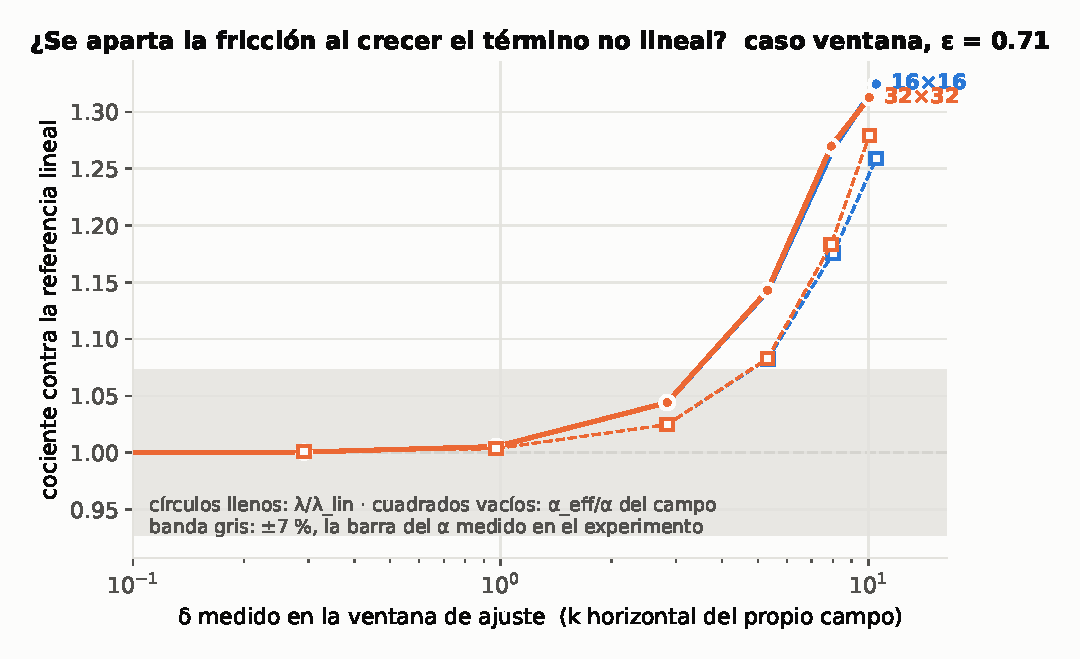
\includegraphics[width=.49\textwidth]{f7_barrido_delta_ventana.pdf}\hfill
  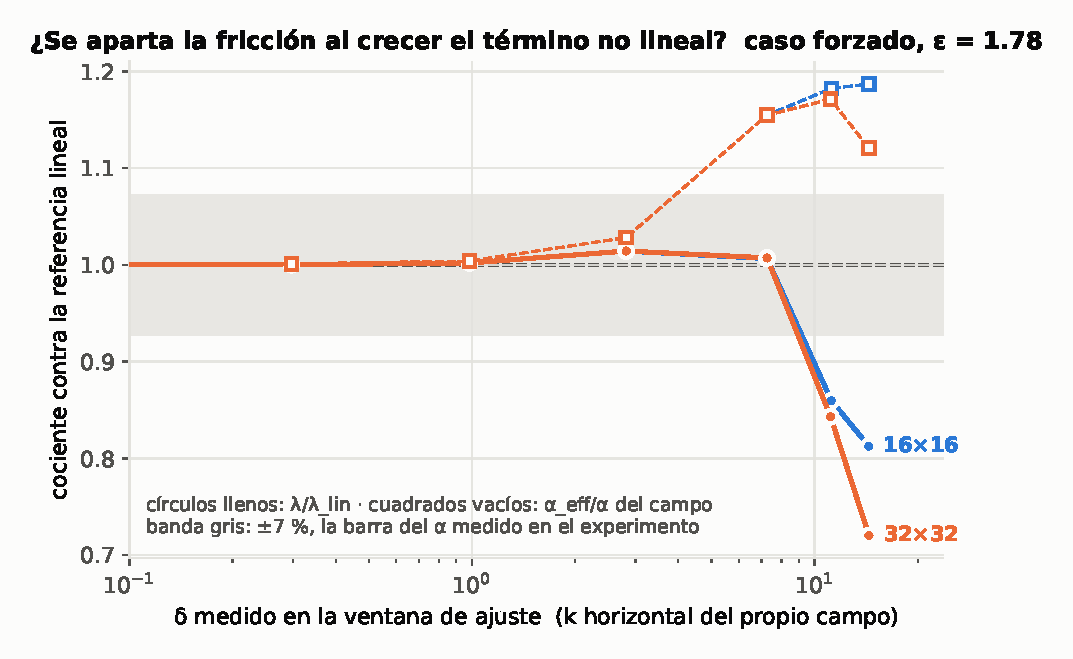
\includegraphics[width=.49\textwidth]{f7_barrido_delta_forzado.pdf}
  \caption{Barrido en $\delta$ \etq{V-16}. Círculos: tasa sobre la lineal; cuadrados:
  $\alpha_{\rm eff}/\alpha$ del campo; banda gris: la barra del $\alpha$ medido en el
  experimento ($\pm7\%$). Izquierda, $\varepsilon=0{,}71$: las dos mallas coinciden
  dentro de $1{,}2\%$ hasta $\delta=10$. Derecha, $\varepsilon=1{,}78$: hasta
  $\delta\approx7$ las mallas coinciden; los dos puntos de más amplitud no convergen y no
  se usan.}
  \label{fig:f7}
\end{figure}

El término no lineal \textbf{sube la fricción de fondo}, en los dos $\varepsilon$:
$2{,}5\%$ en $\delta=3$, $8\%$ en $\delta=5$, $15$--$18\%$ en $\delta\approx7$--$8$,
$26$--$28\%$ en $\delta=10$. El perfil distorsionado tiene más cizallamiento en el fondo
por unidad de velocidad media que el fundamental. La estimación de orden de
§\ref{sec:delta} da el orden y subestima el efecto sobre $\alpha$ por un factor $\sim3$.
Lo que le pasa a la tasa total depende de $\varepsilon$: en $0{,}71$ la fricción domina y
$\lambda$ sigue a $\alpha_{\rm eff}$; en $1{,}78$ la viscosidad horizontal domina y el
término no lineal manda energía a escalas más grandes, que disipan menos, así que la
tasa total queda dentro de $1{,}4\%$ de la lineal mientras $\alpha_{\rm eff}$ subió
$15\%$. Las dos medidas se separan porque miden cosas distintas, y por eso hacía falta
medir las dos. La clausura de un modo queda cuantificada: vale al por ciento para
$\delta\lesssim3$ y hay que corregirla por encima. Procedencia:
\texttt{salidas/tablas/barrido\_delta\_etapa1\_\{ventana,forzado\}.json}; informes con
veredicto automático en \texttt{informe/barrido\_delta\_etapa1\_*.pdf}.

\subsection{Lo que ve un PIV de superficie}
\label{sec:v17}

Sobre las mismas corridas, escribiendo cinco campos dentro de la ventana de ajuste, se
midió la pendiente de $\log u(h)$ ---lo que un PIV ajusta--- contra la de
$\log\avg{u}$ ---lo que predice la clausura---, cada una dividida por la misma tasa en la
referencia lineal \etq{V-17}. Chequeos: la tasa 3D reproduce la de \texttt{balance.txt},
y en la referencia lineal las tres tasas coinciden y $u(h)/\avg u=1{,}5710=\pi/2$ en
los cinco campos.

\begin{center}
\small
\begin{tabular}{ccccccc}
\toprule
$\delta$ & \multicolumn{3}{c}{$\varepsilon=0{,}71$} & \multicolumn{3}{c}{$\varepsilon=1{,}78$}\\
 & $\lambda_{\rm sup}/\lambda_{\rm lin}$ & $\lambda_{\rm prom}/\lambda_{\rm lin}$ & $u(h)/\avg u$
 & $\lambda_{\rm sup}/\lambda_{\rm lin}$ & $\lambda_{\rm prom}/\lambda_{\rm lin}$ & $u(h)/\avg u$\\
\midrule
1 & 1,004 & 1,005 & 1,57 & 1,000 & 1,001 & 1,57\\
3 & 1,033 & 1,040 & 1,56 & 0,996 & 1,011 & 1,55\\
5 & 1,092 & 1,128 & 1,52 & --- & --- & ---\\
7--8 & 1,118 & 1,242 & 1,45 & \textbf{0,891} & 1,013 & 1,44\\
10 & 1,043 & 1,305 & 1,37 & \multicolumn{3}{c}{no convergido entre mallas}\\
\bottomrule
\end{tabular}
\end{center}

\begin{figure}[htbp]
  \centering
  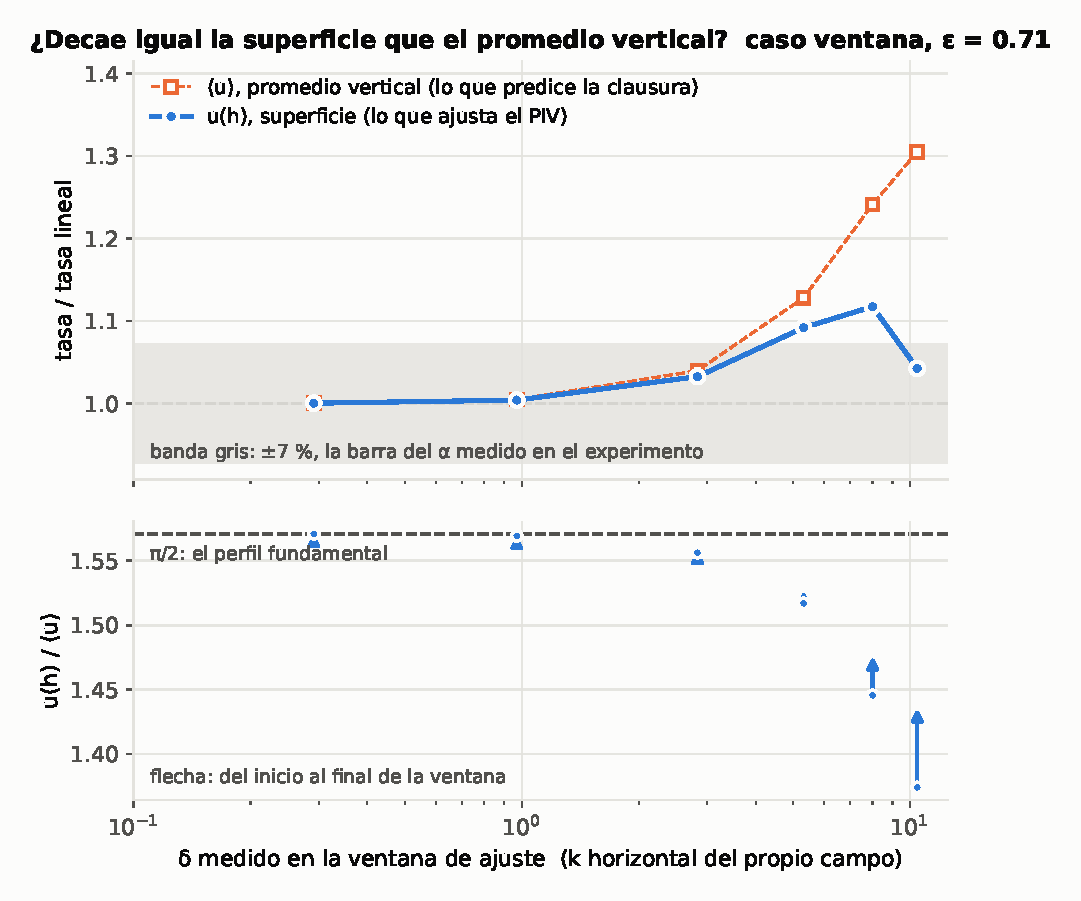
\includegraphics[width=.49\textwidth]{f8_superficie_delta_ventana.pdf}\hfill
  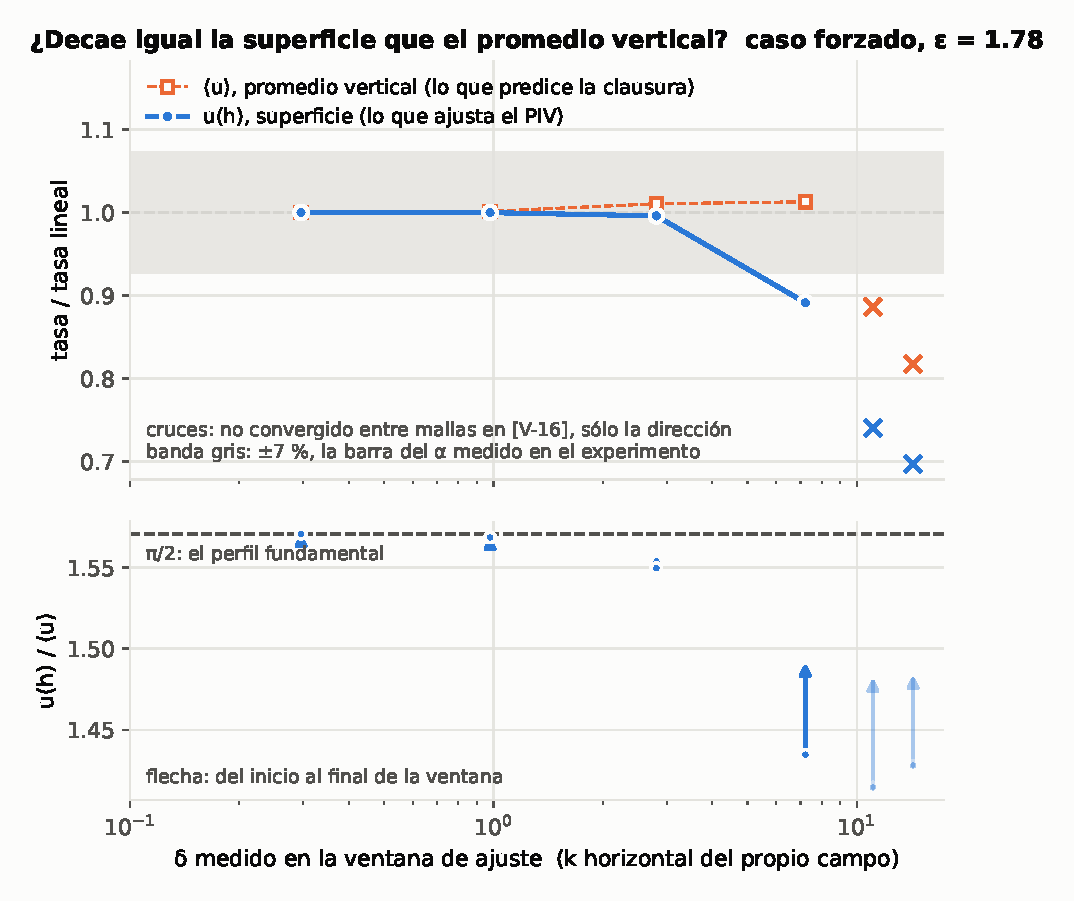
\includegraphics[width=.49\textwidth]{f8_superficie_delta_forzado.pdf}
  \caption{La velocidad de superficie contra el promedio vertical \etq{V-17}. Arriba:
  tasas sobre la lineal; abajo: $u(h)/\avg u$ del inicio al final de la ventana (flecha).
  Izquierda, $\varepsilon=0{,}71$: la tasa del promedio sube hasta $31\%$, la de la
  superficie sólo hasta $12\%$ y nunca baja de la lineal. Derecha,
  $\varepsilon=1{,}78$: la tasa de $u(h)$ cae $11\%$ por debajo de la lineal en
  $\delta=7$; las cruces son los puntos no convergidos, sólo la dirección.}
  \label{fig:f8}
\end{figure}

Tres cosas. (1) El perfil distorsionado tiene menos exceso de superficie: $u(h)/\avg u$
baja de $\pi/2$ a $1{,}37$ en $\delta\approx10$; es el mismo perfil que en
§\ref{sec:v16} tiene más cizallamiento en el fondo. (2) Como $\delta$ cae en el tiempo,
el cociente se recupera hacia $\pi/2$ dentro de la ventana, y por eso $u(h)$ decae más
lento que $\avg u$: $\lambda_{\rm sup}/\lambda_{\rm prom}=0{,}97$ en $\delta\approx5$,
$0{,}90$ en $8$, $0{,}80$ en $10$. Cuenta de control en $\varepsilon=0{,}71$,
$\delta=10{,}4$: $\dd\log(u(h)/\avg u)/\dd t=\ln(1{,}435/1{,}374)/1{,}27=0{,}034$ contra
$\lambda_{\rm prom}-\lambda_{\rm sup}=(1{,}305-1{,}043)\cdot0{,}1308=0{,}034$. (3) En
$\varepsilon=0{,}71$ los dos efectos casi se cancelan: la fricción efectiva sube hasta
$25\%$, pero la tasa de $u(h)$ queda entre $+3$ y $+12\%$ de la lineal hasta
$\delta=10$, nunca por debajo. \textbf{Para un PIV de superficie en el régimen de la
ventana experimental, la predicción lineal \eqref{eq:lamk} es buena al $12\%$ aunque
cada ingrediente no lineal valga 20--30\%}, y la cantidad correcta para comparar es
$\lambda_{\rm sup}$, no $\lambda_{\rm prom}$. En $\varepsilon=1{,}78$ no hay qué
cancelar (la tasa total no sube) y la tasa de $u(h)$ cae $11\%$ por debajo de la
lineal en $\delta=7$. Las pendientes de superficie se midieron sólo en $16^2$; la
convergencia es la de §\ref{sec:v16}.

\section{Contraste con el experimento}
\label{sec:contraste}

La campaña de PIV del 02-06-25 en la celda de forzado electromagnético (cámara Photron
FASTCAM-1024PCI a 60 fps, 3800 px/m, campo de 26,9 cm; capa de 6 mm de KNO$_3$ al
16\% con partículas de 100 $\mu$m; imanes de 1 cm en red tipo tablero de 1,5 cm entre
centros; los parámetros viven en \texttt{codigo/celda.py} con su procedencia \etq{D-27},
\etq{D-41}) tiene cuatro registros de decaimiento libre que forman un \emph{ensemble}:
las barras de error salen de ahí. El ajuste se restringe a $t>10$ s, después de la
meseta inicial, que es el estado forzado previo al corte \etq{D-30}.

\begin{figure}[htbp]
  \centering
  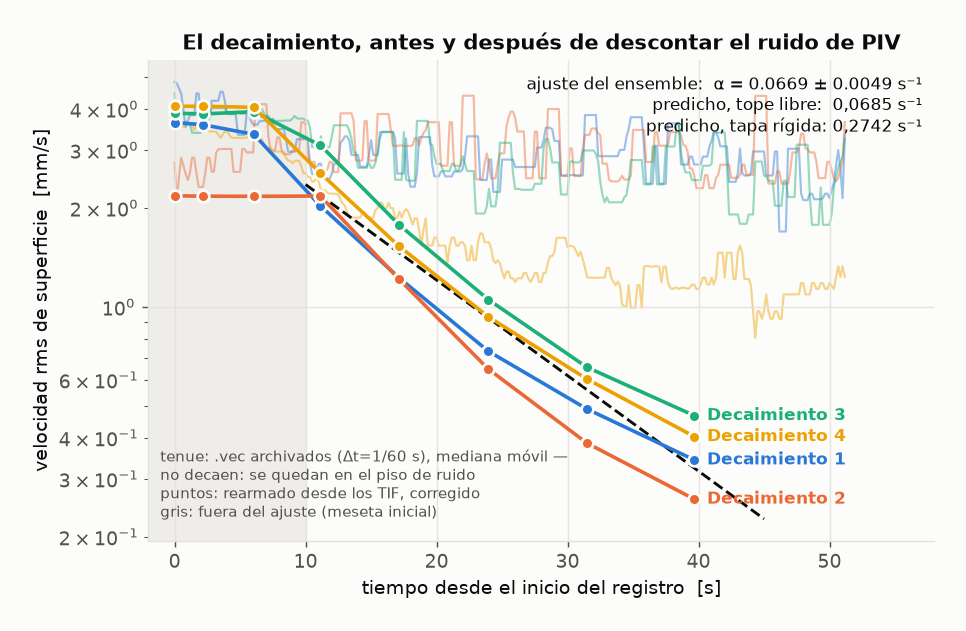
\includegraphics[width=.85\textwidth]{f1_decaimiento_claro.png}
  \caption{El decaimiento, antes y después de descontar el ruido de PIV \etq{V-13}. Las
  series archivadas (trazo tenue) usan pares de cuadros consecutivos, donde el ruido es
  del orden de la señal; reprocesando desde los TIF crudos con $\Delta t$ óptimo y
  multipaso propio (puntos y trazo grueso) el decaimiento exponencial aparece con
  claridad, con $97{,}5\%$ de vectores válidos.}
\end{figure}

\begin{center}
\begin{tabular}{lcc}
\toprule
 & $\alpha$ [s$^{-1}$] & $\tau=1/\alpha$ [s]\\
\midrule
\textbf{medido, ensemble de los 4, $t>10$ s} & $\mathbf{0{,}06687\pm0{,}00488}$ & \textbf{15,0}\\
calculado, superficie libre & 0,06854 & 14,6\\
calculado, tapa rígida & 0,27416 & 3,6\\
\bottomrule
\end{tabular}
\end{center}

El medido queda a $2{,}4\%$ del valor con superficie libre y $4{,}1$ veces por debajo
del de tapa rígida, que es el supuesto de los códigos que hoy usa el grupo. En lo
cualitativo es la comparación que motiva el proyecto: la condición correcta es la
superficie libre, no la tapa rígida. Está limitada por el espesor, no por la
estadística: medio milímetro en $h$ mueve $\alpha$ un $17\%$.

\paragraph{Salvedad cuantitativa, abierta \etq{P-02}.} $\alpha$ pelado es la tasa de un
modo con $k\to0$. Para el $k$ que el flujo sí tiene en la ventana del ajuste
(59--130 m$^{-1}$, medido sobre los espectros) la tasa lineal \eqref{eq:lamk} es
0,072--0,085 s$^{-1}$, y el medido queda un 7--22\% \emph{por debajo}. El barrido en
$\delta$ descartó la no linealidad como explicación (§\ref{sec:v16}: empuja para el otro
lado) y mostró que la cantidad a comparar es la tasa de superficie (§\ref{sec:v17}), que
en este $\varepsilon$ no baja de la lineal. Quedan el contenido en $k$ del campo medido
---el piso de ruido del PIV no es blanco \etq{V-14}--- y el espesor. El $2{,}4\%$ no se
presenta como acuerdo.

\begin{figure}[htbp]
  \centering
  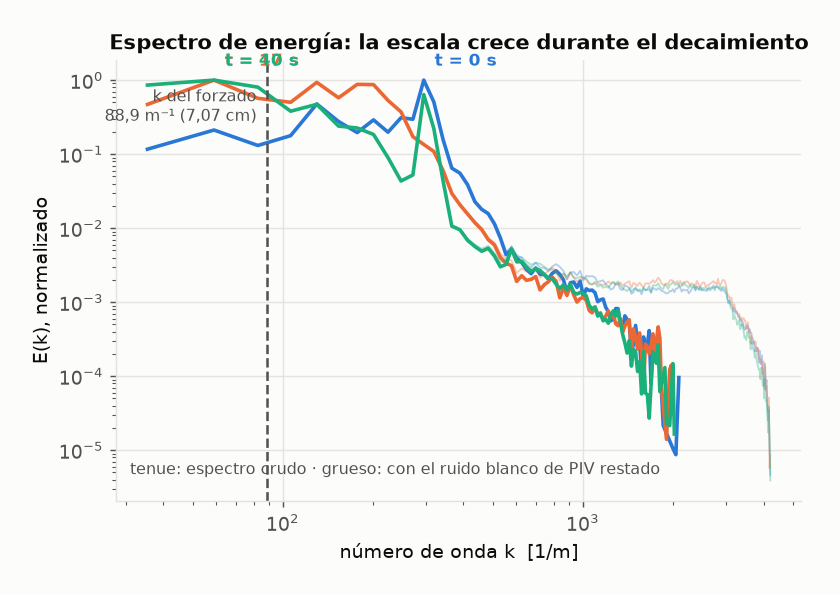
\includegraphics[width=.85\textwidth]{f4_espectros_claro.png}
  \caption{El estado forzado pica en el fundamental de la red de imanes \etq{H-16}: los
  doce espectros de la meseta forzada tienen su pico en 295 m$^{-1}$
  ($\lambda\approx2{,}1$ cm), y la red de 1,5 cm da 296 (línea punteada). Durante el
  decaimiento la escala crece: el número de onda pesado por energía va de 240 m$^{-1}$
  al inicio a 135 al final. Es el $k$ que hay que usar para evaluar $\delta$ y
  $\lambda(k)$ en cada instante.}
\end{figure}

\section{Explorando: preguntas disparadas por los resultados}

Esta zona está en proceso y no es parte del objeto del proyecto. Se muestra porque el
contraste depende de ella y porque documenta lo que se intentó.

\paragraph{El instrumento.} Para que el decaimiento medido sea comparable con algo hizo
falta saber cuánto del valor es ruido de PIV. Se midió $\sigma$ tres veces sobre la misma
cámara y la misma configuración, agregando en cada paso una degradación física: par
sintético con corrimiento conocido, $\le0{,}011$ px \etq{V-04}; fluido en reposo, par
real, $0{,}030$ px; forzado a 2,15 A, ajuste del barrido en $\Delta t$, $0{,}169$ px
\etq{H-05}. El término que agrega el flujo es el $98\%$ de la varianza \etq{H-07}: el
ruido de PIV no es una constante del instrumento, cae junto con el flujo. Lo abierto: el
$0{,}169$ px se midió sobre un registro que resultó no ser estacionario \etq{H-12}, y el
marco espectral de Foucaut \emph{et al.}\ no describe el ruido de este multipaso
\etq{V-14}. Repetir la medición sobre \texttt{med\_S0002}, la corrida forzada que sí es
estacionaria, cerraría el número; es instrumento, no objeto.

\paragraph{Cuánta energía sobrevive en el fundamental de la red.} La salvedad \etq{P-02}
se decide en el contenido en $k$ del campo medido dentro de la ventana. El barrido dice
que en $\varepsilon=1{,}78$ la tasa de superficie sí cae por debajo de la lineal; cuánto
de ese modo queda al comienzo de la ventana es medible sobre los espectros ya guardados y
no se hizo.

\section{Salvedades}

Límites reales del resultado, declarados porque el proyecto no afirma más de lo que se
chequeó.
\begin{itemize}
  \item \textbf{La viscosidad usada es la del agua}, no la del electrolito al 16\%
  \etq{D-27}. Entra a primer orden en $\alpha\propto\nu/h^2$.
  \item \textbf{El espesor domina el error del contraste}: medio milímetro sobre 6 mm
  mueve $\alpha$ un $17\%$.
  \item \textbf{La comparación cuantitativa con el experimento está abierta} \etq{P-02},
  §\ref{sec:contraste}.
  \item \textbf{La puerta no verifica el régimen no lineal}: sus casos usan el modo de
  corte puro, donde el término no lineal es cero; la convergencia en régimen no lineal se
  estudió aparte \etq{V-16}, \etq{H-09} y sólo hasta $\delta\approx7$--$10$. Para producción
  hace falta el estudio de convergencia propio.
  \item \textbf{El barrido es de decaimiento libre}, con dos modos horizontales como
  condición inicial: la meseta forzada no se simuló como estado forzado, ni se usó un
  campo de banda ancha.
  \item \textbf{Sólo doble precisión y Runge--Kutta de orden 2}; con 1, 2 y 4 procesos
  MPI sí está verificado.
  \item \textbf{Una película superficial no se incluye.} Un electrolito con partículas
  flotando podría formar una película que vuelve el tope casi rígido; está modelada como
  condición de Robin con un parámetro \etq{D-29}. No ocurre en este montaje ni es relevante
  para el caso de estudio \etq{D-46}.
\end{itemize}

\section{Qué sigue}

La herramienta ya existe: SPECTER puede calcular la fricción de fondo con superficie
libre en vez de ajustarla, y decir qué le hace la no linealidad. Falta:
\begin{enumerate}
  \item la \textbf{corrida de producción} en el clúster con la geometría real de la
  celda, y de ahí el $\alpha$ calculado con su corrección no lineal; la resolución sale
  del barrido ($32^2$ alcanza hasta $\delta\approx7$ en $\varepsilon=1{,}78$ y hasta
  $\delta\approx10$ en $0{,}71$), y para $\delta$ mayor hace falta el estudio de
  convergencia propio, ya planificado;
  \item la \textbf{superficie deformable} (§\ref{sec:deformable}), como continuación
  después de esta entrega.
\end{enumerate}

\appendix

\section{Reproducir}

Todo lo numérico corre en cualquier máquina sin datos externos. Fuera del repositorio
quedan, a propósito, el árbol de SPECTER (se reconstruye desde upstream con el parche),
los PDF de la bibliografía y los datos crudos del PIV (140 GB, sólo lectura).
{\small\begin{verbatim}
git clone https://github.com/Lucia-Maz/\
          free-slip-boundary-conditions-fourier-continuation.git
mamba create -n piv-dt -c conda-forge python=3.11 numpy scipy matplotlib \
      tifffile imageio scikit-image pip && pip install openpiv
mamba create -n specter -c conda-forge gfortran openmpi openmpi-mpifort fftw make
git clone https://github.com/mfontanaar/SPECTER.git numerico/SPECTER-upstream
cd numerico/SPECTER-upstream && git checkout 0ad1edb && cd ../..
cp -r numerico/SPECTER-upstream numerico/SPECTER-trabajo
cd numerico/SPECTER-trabajo && git apply ../specter-parche/superficie-libre.patch
cp ../specter-parche/laplace_dirneu.f90 src/tests/ && cd ../..
python verificacion/test_aceptacion_fase1.py            # 6/6, segundos
python verificacion/test_aceptacion_fase2.py            # 6/6, ~10 min
python verificacion/barrido_delta_etapa1.py --caso ventana --resolucion 16
python verificacion/barrido_delta_etapa1.py --caso ventana --resolucion 16 --superficie
\end{verbatim}}
Las convenciones del proyecto ---qué no se hardcodea, qué no se edita, qué no se afirma
sin chequear--- están en \texttt{CLAUDE.md}, y valen igual en la laptop y en el clúster.

\section{Procedencia de cada número}

\begin{center}
\small
\begin{tabular}{p{4.2cm}p{10.5cm}}
\toprule
número & de dónde sale\\
\midrule
$\alpha=\nu\pi^2/4h^2$, factor 4, $\pi/2$ & \path{verificacion/test_aceptacion_fase1.py}; \path{jobs/.../out/build/notes.pdf}, \path{out/provenance.json}; \etq{V-07}\\
error $6{,}8\cdot10^{-10}$, residuo $6{,}1\cdot10^{-12}$ & \path{verificacion/test_aceptacion_fase2.py}, casos V4 y V3; \etq{V-09}\\
$\eta/h$, Froude & \path{numerico/fase4/superficie_libre_escalas.py} $\to$ \path{salidas/tablas/superficie_libre_escalas.json}; \etq{D-28}\\
$\varepsilon$, $\delta$, distorsión & \path{numerico/fase4/p01_validez.py} $\to$ \path{salidas/tablas/p01_validez.json}; \etq{V-11}, \etq{D-41}\\
$\alpha_{\rm eff}/\alpha$, $\lambda/\lambda_{\rm lin}$ & \path{verificacion/barrido_delta_etapa1.py} $\to$ \path{salidas/tablas/barrido_delta_etapa1_*.json}; \etq{V-16}\\
$\lambda_{\rm sup}$, $\lambda_{\rm prom}$, $u(h)/\avg u$ & el mismo script con \path{--superficie} $\to$ \path{..._superficie.json}; \etq{V-17}\\
$\alpha$ medido, espectros & \path{codigo/06_decaimiento.py} $\to$ \path{salidas/tablas/decaimiento.json}, \path{decaimiento_resumen.json}; \etq{V-13}, \etq{H-16}\\
$\sigma$ del PIV & \path{codigo/02}, \path{04}, \path{05} $\to$ \path{salidas/tablas/}; \etq{V-04}, \etq{H-05}, \etq{H-07}\\
\bottomrule
\end{tabular}
\end{center}

\begin{thebibliography}{9}
\bibitem{fontana2020} M.~Fontana, O.~P.~Bruno, P.~D.~Mininni y P.~Dmitruk,
\emph{Fourier continuation method for incompressible fluids with boundaries},
Comput.\ Phys.\ Commun.\ \textbf{256}, 107482 (2020),
\href{https://doi.org/10.1016/j.cpc.2020.107482}{10.1016/j.cpc.2020.107482}. Leído en el
original \etq{V-08}. Los demás trabajos citados en el repositorio, con DOI resueltos
contra Crossref, están en \texttt{bibliografia/REFERENCIAS.md}.
\end{thebibliography}

\end{document}
